\documentclass[10pt,a4paper]{article}

\usepackage{amssymb}
\usepackage[english]{babel}
\usepackage[utf8]{inputenc}
\usepackage{graphicx}
\usepackage{lineno}
\usepackage{cite}
\usepackage{float}
\usepackage{ccaption}
\usepackage{caption}
\usepackage{array}
\usepackage{lscape}
\usepackage[hmargin=2cm,vmargin=2cm]{geometry}
\usepackage{fancyvrb}
\usepackage{hyperref}

\title{{\tt TESS3} reference manual \\
Command-line program and R wrapper functions
}

\author{
        Kevin Caye (kevin.caye@imag.fr)\\
        Olivier Fran\c cois (olivier.francois@imag.fr)\\
}

\newcommand{\bp}{\mathbf{p}}
\newcommand{\LLL}{\mathcal{L}}

%% BEGIN DOC
\begin{document}


\maketitle
\begin{center}
{\it Please, print this reference manual only if it is necessary.}
\end{center}

\vspace{.5cm}

\begin{center} {\bf Summary}
\end{center}


\vspace{.5cm}

Geography is an important determinant of genetic variation in natural populations, and its effects are commonly investigated by analyzing population genetic structure using spatial ancestry estimation programs. A common issue is that classical spatial ancestry estimation programs do not scale with the dimension of the data sets generated from modern sequencing technologies, and more efficient algorithms are needed to analyze genome-wide patterns of population genetic variation in their geographic context.

The computer program {\tt TESS3}, which has functionalities similar to the previous versions of {\tt TESS}~\cite{chen2007bayesian,durand2009spatial}, has run-times several order faster than those of common Bayesian clustering programs. In addition, the program can be used to perform genome scans for selection based on ancestral allele frequency differentiation statistic, and to separate non-adaptive and adaptive genetic variation.

This documentation aims to help users to run the {\tt TESS3} command-line engine on Linux, Mac and Windows operating systems, and presents some R functions that facilitate the post-processing of the program outputs. The main features of {\tt TESS3} are illustrated using an example data set, simulated from European lines of the plant species {\it Arabidopsis thaliana}.

\vspace{.5cm}


\section{Program installation} 

The installation of {\tt TESS3} requires that {\tt CMake}, a the cross-platform open-source build system, is installed on the computer OS (\url{ http://www.cmake.org/}).  The {\tt TESS3}  program source code can be downloaded from the following Github address: \url{https://github.com/cayek/TESS3}. After downloading the files as a zipped archive, unzipping the archive will create a {\tt TESS3-master} directory on the system. This  directory contains the following subdirectories:
\begin{itemize}
\item   {\tt src}: the source code of the program,

\item   {\tt external}: external libraries,

\item   {\tt tutorial}: {\tt R} scripts that run example data analysis with the TESS3 program.

\item     {\tt doc}: the program documentation.

\item     {\tt data}: some simulated data sets for experimenting the program use.
\end{itemize}
\noindent The installation of {\tt TESS3} can be performed by typing the following instructions in a terminal session from the {\tt TESS3-master} directory.

\begin{Verbatim}[frame = single]
 mkdir build/
 cd build/
 cmake -DCMAKE_BUILD_TYPE=release ../
 make TESS3
\end{Verbatim}

 \noindent The executable program file {\tt TESS3} will be found in the {\tt build} directory. Copy this file to the \verb|TESS3-master| directory, and change directory to the main directory.
  
\section{Data format}

\subsection{Input files}

{\tt TESS3} requires two input files, the first one recording individual genotype data and the second one containing the geographic coordinates of  each sampled individual. For organism genomes of arbitrary ploidy, the standard data type for {\tt TESS3} is the {\bf single nucleotide polymorphism} (SNP) type.  The genotype matrix must be formatted in the {\bf geno} format and the coordinate file must be formatted in the {\bf coord} format.

Users who want to process allelic data, such as microsatellite markers or AFLPs, and have their data in the {\tt TESS} 2.3 format can also use {\tt TESS3}. They need to convert their data in the geno+coord data format, and can do this using the {\tt tess2tess3} function implemented in the {\tt R} script {\tt src/Rwrapper/TESS3.R}.




\begin{itemize}
\item {\bf geno} (example.geno)

The {\bf geno} format has one row for each SNP. Each row contains 1 character per individual. For diploid genomes,  0 means zero copies of the reference allele, 1 means one copy of the reference allele, 2 means two copies of the reference allele, and 9 codes for some missing data. Here is an example of a geno file for $n=3$ individuals and $L=4$ loci.
\\
\begin{center}
\footnotesize
\begin{Verbatim}[frame=single]
112
010
091
121
\end{Verbatim}
\end{center}


\item {\bf coord} (example.coord)

The {\bf coord} format has one row for each individual. Each row contains the \verb|longitude| and \verb|latitude| coordinates of each individual.
\\
\begin{center}
\footnotesize
\begin{Verbatim}[frame=single]
2.5154 5.4390
-8.4293 4.0197
1.3536 5.5852
\end{Verbatim}
\end{center}

\end{itemize}

\noindent Users having their genotype data in the {\bf ped}, {\bf ancestrymap}, {\bf vcf} or {\bf lfmm} format  can use the {\tt R} package {\tt LEA} to convert them in the {\bf geno} format~\cite{frichot2015lea}. 

\subsection{Output files}

{\tt TESS3} produces three main {\bf output files}:

\begin{itemize}
\item The file with the extension the {\bf .K.Q} contains the $Q$-matrix of individual ancestry coefficients.
The $Q$-matrix has $n$ rows (the number of individuals) and $K$ columns (the number of ancestral populations).
\item The file with the extension {\bf K.G} contains the $G$-matrix of ancestral genotype frequencies.
The $G$-matrix has $N_g\times L$ lines (the number of genotypes times the number of SNPs) and $K$ columns (the number of ancestral populations). For diploid organisms, the first row represents the frequencies of genotype 0 in each ancestral population, the second row represents the frequencies of genotype 1, and the third line the ancestral frequencies of 2.
\item The file with the extension {\bf .Fst} contains the values of the ancestral allele frequency differentiation statistic $F_{\rm ST}$ computed at each locus.  
\end{itemize}

There are additional {\bf output files} that are useful to get information about the nearest-neighbor graph, the least-squares error and the cross-entropy criterion computed by the program.

\begin{itemize}
\item The file with the extension {\bf .W} contains weight matrix for the nearest-neighbor graph.
\item The file with the extension the {\bf .sum} contains the values of the least-squares error, the cross-entropy criterion computed with all the data and with a percentage of masked data when the user asks the program to compute it.
\end{itemize}

\section{Run the program}
\subsection{Command-line}
The {\tt TESS3} program can be executed from a command line. The basic format is as follows
\begin{Verbatim}[frame=single]
./TESS3 -x genotype_file.geno  -r coordinates_file.coord -K number_of_ancestral_populations
\end{Verbatim}

\noindent
Only the three options {\tt -x -r -K}  are mandatory. The ordering of the options in the command line is unimportant. Here is a description of these options:
\begin{itemize}
\item \verb|-x genotype_file.geno| is the path to the genotype file (in the .geno format),
\item \verb|-r coordinates_file.coord| is the path to the coordinate file (in the .coord format),
\item \verb|-K number_of_ancestral_populations| is the number of ancestral populations.
\end{itemize}

\noindent
Some additional options are available:
\begin{itemize}
\item \verb|-m ploidy|  1 if haploid, 2 if diploid (default: 2). 
\item \verb|-a alpha| is the value of the normalized regularization parameter (default: 0.001). This parameter controls the geographic regularity of ancestry estimates.
\item \verb|-W edge_weight_input| is the path to a file that contains a pre-specified edge weight matrix for the nearest-neighbor graph (separator = space character). The program uses this matrix when the option is set, otherwise it uses the default values.
\item \verb|-q output_Q| is a path for the output file containing the $Q$-matrix of ancestry coefficients. The default name of the output file is the same name as the input file with the extension {\tt .K.Q}.
\item \verb|-g output_G| is a path to the output file containing the ancestral genotype frequencies. The default name of the output file is the same name as the input genotype file with the extension {\tt .K.G}.
\item \verb|-f output_FST| is a path to the output file containing the values of the ancestral allele frequency differentiation statistic for each loci. The default name of the output file is the same name as the input genotype file with the extension {\tt .K.Fst}.
\item \verb|-y output_sum| is a path to the output file containing the value of the least-squares criterion, the cross-entropy criteria on all data and on masked data only. By default, the name of the output file is the same name as the input genotype file with the extension {\tt .K.sum}.
\item \verb|-c perc| is the percentage of masked genotypes. If this option is set, the cross-entropy criterion is computed (see\cite{frichot2014fast} for more details on the cross-entropy criterion). The default percentage is $0.05$.
\item \verb|-e tolerance| is the tolerance error in the optimization algorithm (by default: 0.0000001). 
\item \verb|-i iteration_number| is the maximum number of iterations of the algorithm (default: 200). 
\item \verb|-I nb_SNPs| starts the algorithm with a run using a subset of nb\_SNPs random SNPs. This option speeds up the estimation algorithm for very large data sets.
\item \verb|-Q input_Q| is the path to an initial file for the $Q$ matrix containing individual ancestry coefficients. If both \verb|-I| and \verb|-Q| are set, \verb|-Q| is chosen.
\item \verb|-s seed| is a seed to initialize the random number generator. 
\item \verb|-p p| is the number of CPUs to use when the algorithm is run on a multiprocessor system.
Be aware that the number of processes has to be lower or equal to the number of CPU units available on your computer (default: 1).

\end{itemize}


\noindent A summary of options can be obtained  by typing the following command
\footnotesize
\begin{Verbatim}[frame=single]
./TESS3 -h
\end{Verbatim}
\noindent
\normalsize


\subsection{Example}\label{sec:ex}

To run a very simple example of the use of {\tt TESS3}, consider data simulated from the chromosome 5 of the model plant species {\it A. thaliana}. The genotype matrix contains 170 genotypes from European lines of the plant (26943 SNPs). Since {\it A. thaliana} is a selfing species, the heterozygote frequency was equal to zero, and the diploid genotypes were recoded as haploid. Copy the program executable file in the {\tt ./data/simulated/Athaliana} directory and type

\begin{Verbatim}[frame=single]
./TESS3 -x Athaliana.geno  -r Athaliana.coord -K 3 -m 1
\end{Verbatim}

\noindent Then, open a {\tt R} session and type


\begin{Verbatim}[frame=single]
> par( mfrow = c(2,1) )
> Qmatrix = t( read.table("Athaliana.3.Q") )
> barplot(Qmatrix, col = 2:4)
> Fst = read.table("Athaliana.3.Fst")[,1]
> plot(Fst, main = "Manhattan Plot", cex = .4, pch = 19, col = "blue")
\end{Verbatim}

Those commands visualize the ancestry coefficient matrix computed by {\tt TESS3} and display a Manhattan plot of $F_{\rm ST}$ values along the fifth chromosome of the plant species (figure~\ref{fig:bar}).


\begin{figure}[h!]\centering
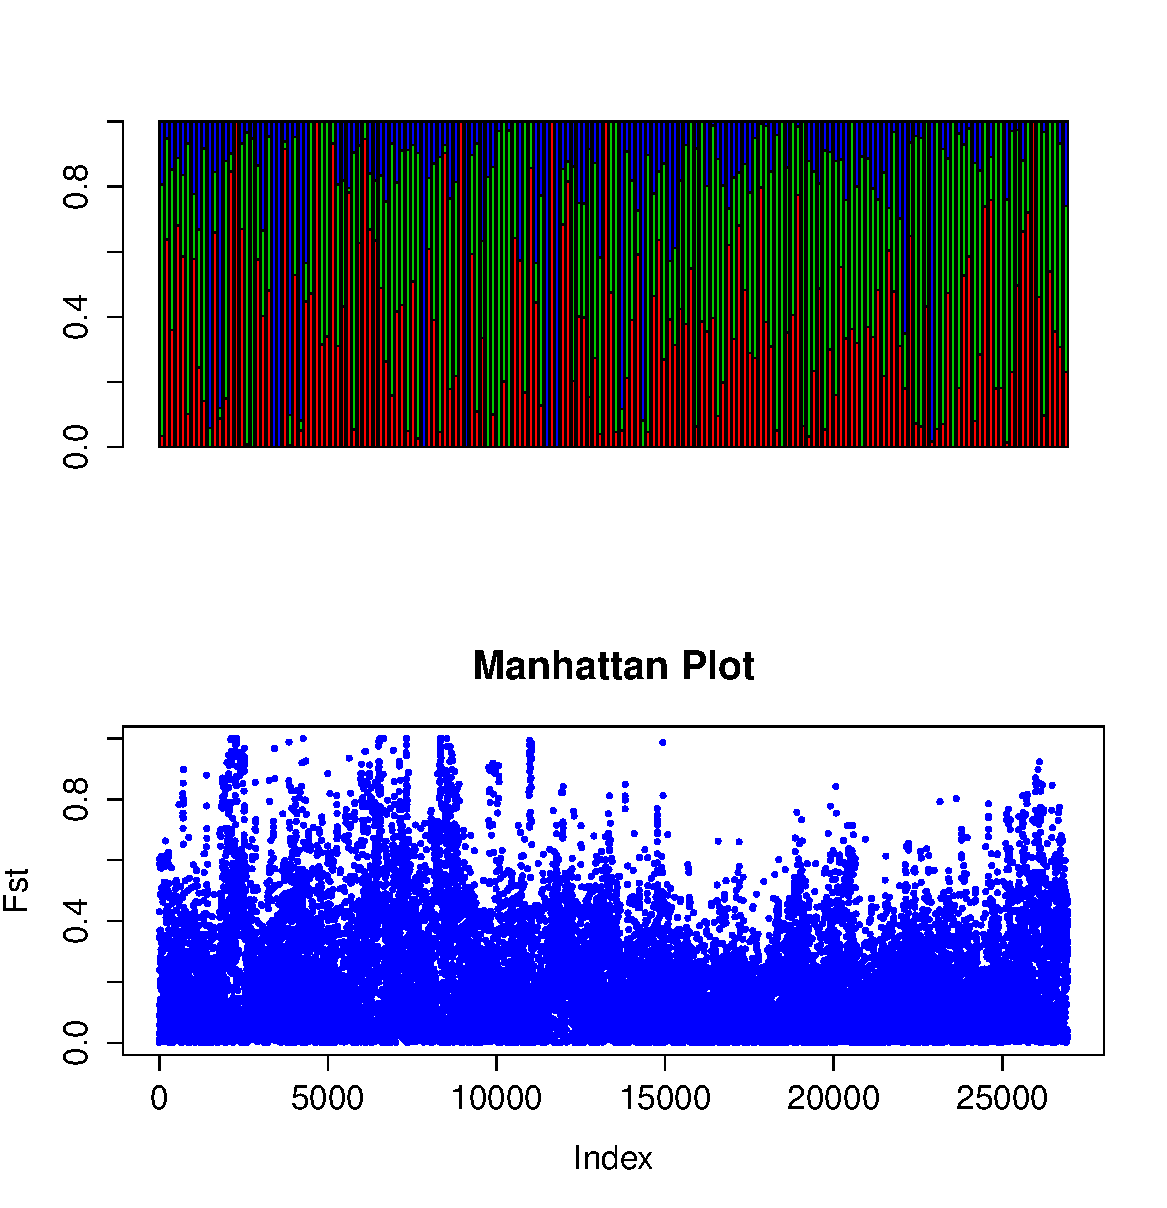
\includegraphics[width=\linewidth]{barplot.pdf}
\caption{Results of the {\tt R} commands of section 3.2.}\label{fig:bar}
\end{figure} 

\subsection{R wrapper functions}
To facilitate the interpretation of results, the {\tt TESS3} program can be launched from the {\tt R} command line directly. This can be done by using the functions in the  \verb|src/Rwrapper/TESS3.R| script. Users need a compiled version of {\tt TESS3} and can use the bash script \verb|./setupRsrc.R| in the {\tt TESS3-master} directory to set the path variables in the R script:
\begin{Verbatim}[frame=single]
./setupRsrc.sh
\end{Verbatim}
Then users need to open an {\tt R} session in the main directory {\tt TESS3-master} and source the \verb|src/Rwrapper/TESS3.R| script as follows: 
\begin{Verbatim}[frame=single]
>source("./src/Rwrapper/TESS3.R")
\end{Verbatim}
The main {\tt R} functions are described below.


\begin{itemize}

\item \verb|TESS3|

\paragraph{Description:}
A wrapper function that calls the {\tt TESS3} command-line program. This function creates a directory named \verb|TESS3_workingDirectory| to record all output files. The function returns an object of class \verb|tess3| which stores the results of the runs. Results can be retrieved thanks to the "getter" functions described below.
\paragraph{Usage}
\begin{Verbatim}
object = TESS3( genotype,
                coordinates,
                K,
                ploidy=1,
                seed=-1, 
                rep = 1, 
                maskedProportion = 0.0, 
                alpha = 0.001 )
\end{Verbatim}
\paragraph{Arguments}
\begin{itemize}
\item \verb|genotype|: a path to a genotype matrix in the {\bf geno} format or directly a {\tt R} genotype matrix of size $n$ individuals by $L$ loci. 
\item \verb|coordinates|: a path to a spatial coordinate matrix in the {\bf coord} format or directly a {\tt R} coordinates matrix of size $n$ by $2$. 
\item \verb|K|: number of ancestral cluster. It can be a sequence of integer values. The {\tt TESS3} program will be run for each element in the sequence.
\item \verb|ploidy|: 1 if haploid, 2 if diploid.
\item \verb|rep|: number of runs for each value of $K$.
\item \verb|maskedProportion|: if \verb|maskedProportion > 0|, the cross-entropy criterion is computed for this percentage of masked genotypes.
\item \verb|alpha|: value of the normalized regularization parameter. This parameter controls the spatial regularity of the ancestry estimates.
\end{itemize}

\paragraph{Value}
\verb|TESS3| returns an object of class "\verb|tess3|". The object contains one list for each run, with the following components: 

\begin{itemize}
\item \verb|Q|: a list containing the $Q$-matrix of ancestry coefficients for each repetition of the algorithm.
\item \verb|G|: a list containing the $G$-matrix of ancestral genotype frequency for each repetition of the algorithm.
\item \verb|Fst|: a list containing the vector of ancestral allele frequency differentiation statistics for each repetition of the algorithm.
\item \verb|error|: a vector containing the residual errors for each repetition of the algorithm.
\item \verb|masked.ce|: if it was computed, a vector containing the value of the cross-entropy criterion for each repetition of the algorithm.
\end{itemize}


\item \verb|Getter functions|

\paragraph{Description}
Functions useful to retrieve the results of the {\tt TESS3} runs. These functions must be used with an object of class \verb|tess3| (see description above).

\begin{itemize}
  \item[] \verb|qmatrix| gets the $Q$-matrix of ancestry coefficients.
  \item[] \verb|gmatrix| gets the $G$-matrix of ancestral genotype frequencies.
  \item[] \verb|fst| gets the vector of $F_{\rm st}$ statistics from each locus.
  \item[] \verb|cross.entropy| if it has been computed, get the vector of cross entropy criterion from each run.
  \item[] \verb|residual.error| gets the vector of the residual errors from each run.
\end{itemize}


\paragraph{Usage}
\begin{Verbatim}
qmatrix( object, K, run = "best" )
 
gmatrix( object, K, run = "best" )
  
fst( object, K, run = "best" )
  
cross.entropy( object, FUNCTION = mean ) 

residual.error( object, FUNCTION = mean )

\end{Verbatim}
\paragraph{Arguments}
\begin{itemize}
\item \verb|object|: an object returned by the \verb|TESS3| function.
\item \verb|K|: number of ancestral cluster.
\item \verb|run|: number of the run, or \verb|"best"| if the best result with respect to the least-squares criterion is desired.
\item \verb|FUNCTION|: function used to summarize data over all run.

\end{itemize}

\paragraph{Value}
\verb|qmatrix| returns an object of class \verb|qmatrix| containing the following components: 

\begin{itemize}
\item \verb|Q|: the $Q$-matrix of ancestry coefficients.
\item \verb|K|: the number of ancestral cluster.
\end{itemize}

\verb|gmatrix| returns an object of class \verb|gmatrix| containing the following components: 

\begin{itemize}
\item \verb|G|: the $G$-matrix of ancestral genotype frequency.
\item \verb|K|: the number of ancestral cluster.
\end{itemize}

\verb|fst| returns an object of class \verb|fstmatrix| containing the following components: 

\begin{itemize}
\item \verb|Fst|: the vector of $F_{\rm st}$ statistics for each locus.
\item \verb|K|: the number of ancestral cluster.
\end{itemize}

\verb|cross.entropy| returns the vector of cross entropy criterion for each run.

\verb|residual.error| returns the vector of residual errors for each run.

\item \verb|Conversion function|

\paragraph{Description}
Functions used to convert data from {\tt TESS} 2.3 format to geno+coord format.

\begin{itemize}
  \item[] \verb|tess2tess3| converts a file in the {\tt TESS} 2.3 data format into geno+coord files which can be used with {\tt TESS3}.
\end{itemize}

\paragraph{Usage}
\begin{verbatim}
tess2tess3( file )
\end{verbatim}
\paragraph{Arguments}
\begin{itemize}
\item \verb|file|: name of the file to convert.
\end{itemize}

\paragraph{Example}
The file {\tt data.tess} used in this example is available in the directory {\tt data/simulated/simpleTESS2}.
\begin{verbatim}
# Will create the coordinate.coord and genotype.geno file from the file data.tess
tess2tess3( "data.tess" ) 
\end{verbatim}

\end{itemize}





\section{Tutorial}


\subsection{Data set}

We illustrate the use of {\tt TESS3} and the {\tt R} functions using simulated {\it Arabidopsis thaliana} data as in sections~\ref{sec:ex} ~\cite{atwell2010genome}. We consider a data set of $n = 170$ (haploid) individuals genotyped at $L = 26943$ SNPs. Open a {\tt R} session from the {\tt TESS3-master} directory.

\subsection{Example of visualization of ancestry coefficients using {\tt TESS3}}\label{sec:struc}

This example describes how to run {\tt TESS3} from the {\tt R} command line for several values of the number of ancestral populations, and how to plot a graph of the cross-entropy criterion as function of $K$ (Figure~\ref{fig:map}). It also uses scripts available from {\tt POPS} web-site (\url{http://membres-timc.imag.fr/Olivier.Francois/pops.html}) to display geographic representations of ancestry coefficient maps using raster files \cite{jay2012forecasting} (Figure~\ref{fig:map}). 

\begin{Verbatim}[frame=single]
Athaliana.directory <- "./data/simulated/Athaliana"

setwd( Athaliana.directory )
###########################################################################
# Run TESS3 on a data set simualted from an Arabidopsis Athalina data set #
###########################################################################

#read data
spatialData = read.coord("Athaliana.coord")
n = nrow(spatialData)

project = TESS3( genotype = "Athaliana.geno", 
                 coordinates = "Athaliana.coord", 
                 K = 1:5, 
                 ploidy = 1, 
                 rep = 1, 
                 maskedProportion = 0.2)


###########################################
# Choose K with cross-entropy criterion #
###########################################

plot( 1:5, cross.entropy( project ), main  = "Cross Entropy",type="b", 
      xlab = "K", ylab = "cross entropy" )

################################
# Plot result on map for K = 3 #
################################

# pops R scripts
source("../../../src/popsRScripts/POPSutilities.r") # WARNING: this 
script may require to be sourced twice!

asciiFile="lowResEurope.asc"
grid=createGridFromAsciiRaster(asciiFile)
# Display only altitudes above sea level
constraints=getConstraintsFromAsciiRaster(asciiFile,cell_value_min=0)

maps(matrix = qmatrix( project, K = 3 )$Q,
     coord = spatialData,
     grid=grid,constraints=constraints,method="max",main="ancestry coefficient with K = 3")
\end{Verbatim}

%$


\begin{figure}[h!]\centering
\begin{minipage}{0.49\textwidth}
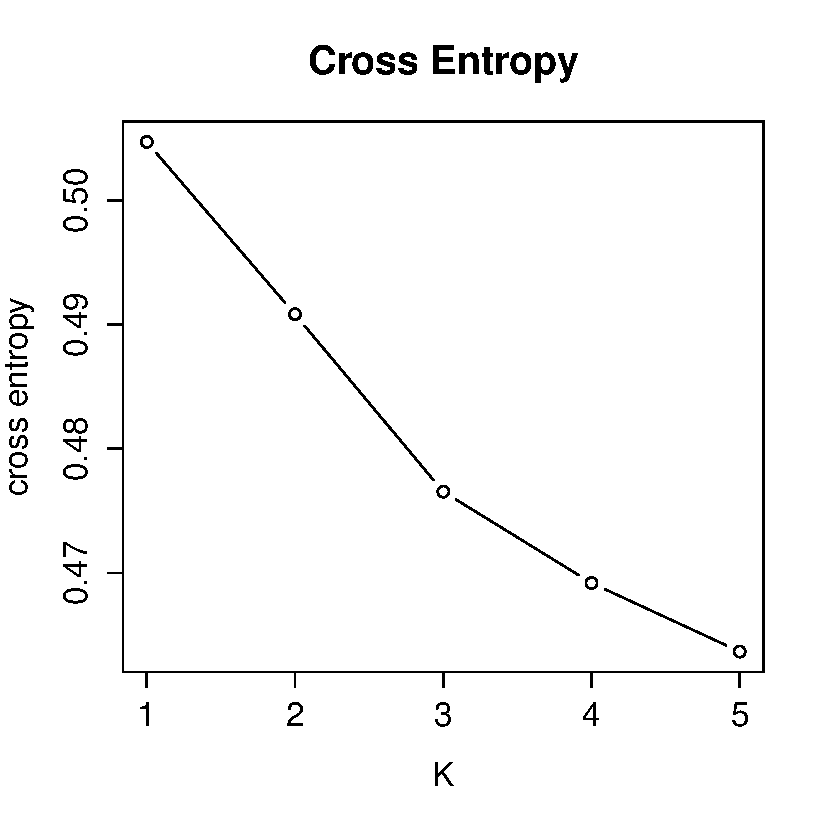
\includegraphics[width=\linewidth]{crossEntropy.pdf}
\end{minipage}
\begin {minipage}{0.49\textwidth}
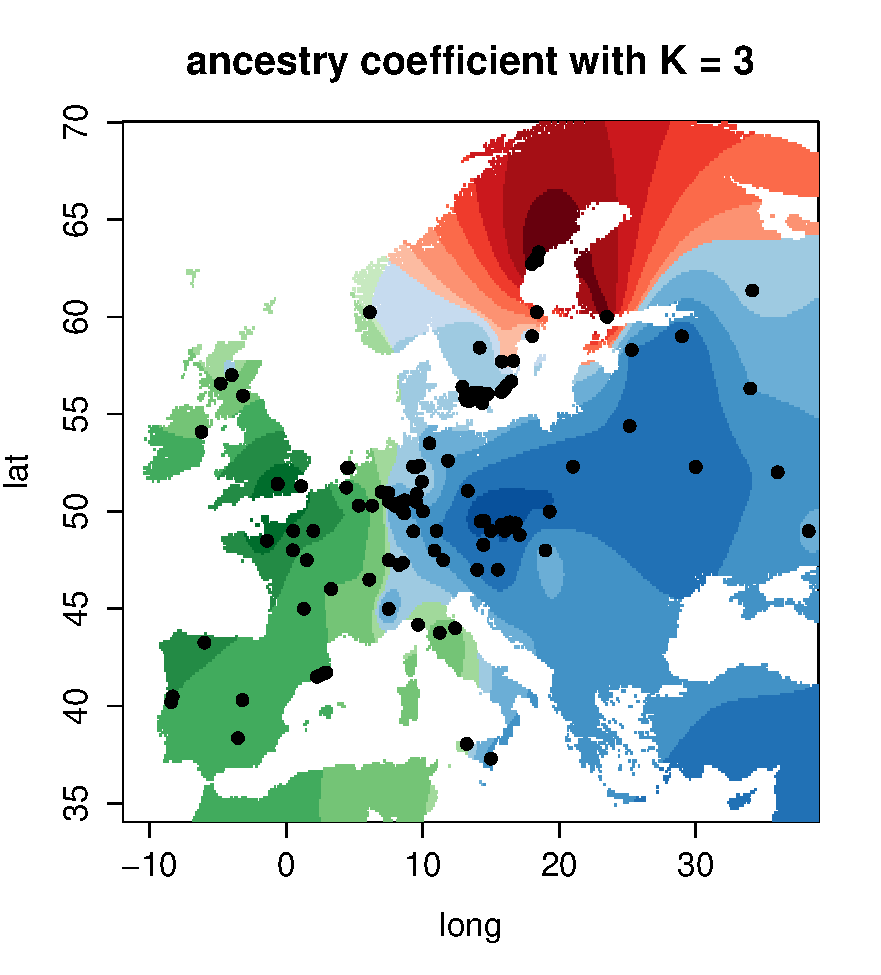
\includegraphics[width=\linewidth]{map.pdf}
\end{minipage}
\caption{Graphs generated with the R script of section~\ref{sec:struc}.}\label{fig:map}
\end{figure} 


\subsection{Example of a genome scan for selection using {\tt TESS3}}\label{sec:sel}
This section shows an example of the use of {\tt TESS3} to perform a genome scan for selection based on the computation of ancestral allele frequency differentiation statistics. Here {\tt TESS3} was run with $K = 3$ ancestral populations. The $F_{\rm ST}$ statistics were transformed into squared $t$-scores and $p$-values using a Fisher distribution. Inflation of the test statistic caused by population structure was corrected by recalibrating the $p$-values to follow a uniform distribution under the null hypothesis. The false discovery rate was controlled using the Benjamini-Hochberg procedure and candidate loci are shown above the green dashed line threshold in the Manhattan Plot (Figure~\ref{fig:manhattanPlot}).

 %% You need to change \verb|TESS3_directory| by the directory path of {\tt TESS3}.

\newpage

\begin{Verbatim}[frame=single]
Athaliana.directory <- "./data/simulated/Athaliana"

setwd( Athaliana.directory )
#####################################################################
# Run TESS3 on data simulated from an Arabidopsis thaliana data set #
#####################################################################

# Read data
spatialData = read.coord("Athaliana.coord")
n = nrow(spatialData)

project = TESS3( genotype = "Athaliana.geno", 
                 coordinates = "Athaliana.coord", 
                 K = 3, 
                 ploidy = 1, 
                 rep = 5 )


#############################
# Genome scan for selection #
#############################

#### Fst with TESS3 
Fst = fst( project, K = 3 )$Fst
Fst[Fst < 0.0] = 0.0

#### Convert Fst into t score
squared.t.scores = Fst*(n-3) / 2 / (1-Fst)

#### Recalibrated p-values
# the gif is set manually 
gif = 12.5
adj.p.values = pf( squared.t.scores/gif , df1 = 2, df2 = n-3, lower = FALSE )

hist(adj.p.values,prob=TRUE)

#### Benjamini Hochberg procedure
alpha = 1e-10
L = length(adj.p.values)
# return a list of candidates with an expected FDR of alpha.
w = which(sort(adj.p.values) < alpha * (1:L) / L)
candidates = order(adj.p.values)[w]
threshold = max(adj.p.values[candidates])

#### Manhattan plot 
plot( 1:length(adj.p.values),-log10(adj.p.values) , 
      main = "Manhattan Plot" , 
      xlab = "indices", 
      ylab="- Log P-value", 
      pch=19, cex = .5) 
#add threshold
abline( -log10(threshold), 0, col = "green", lty = 6, lwd = 3 )
\end{Verbatim}

%$

\begin{figure}[h!]\centering
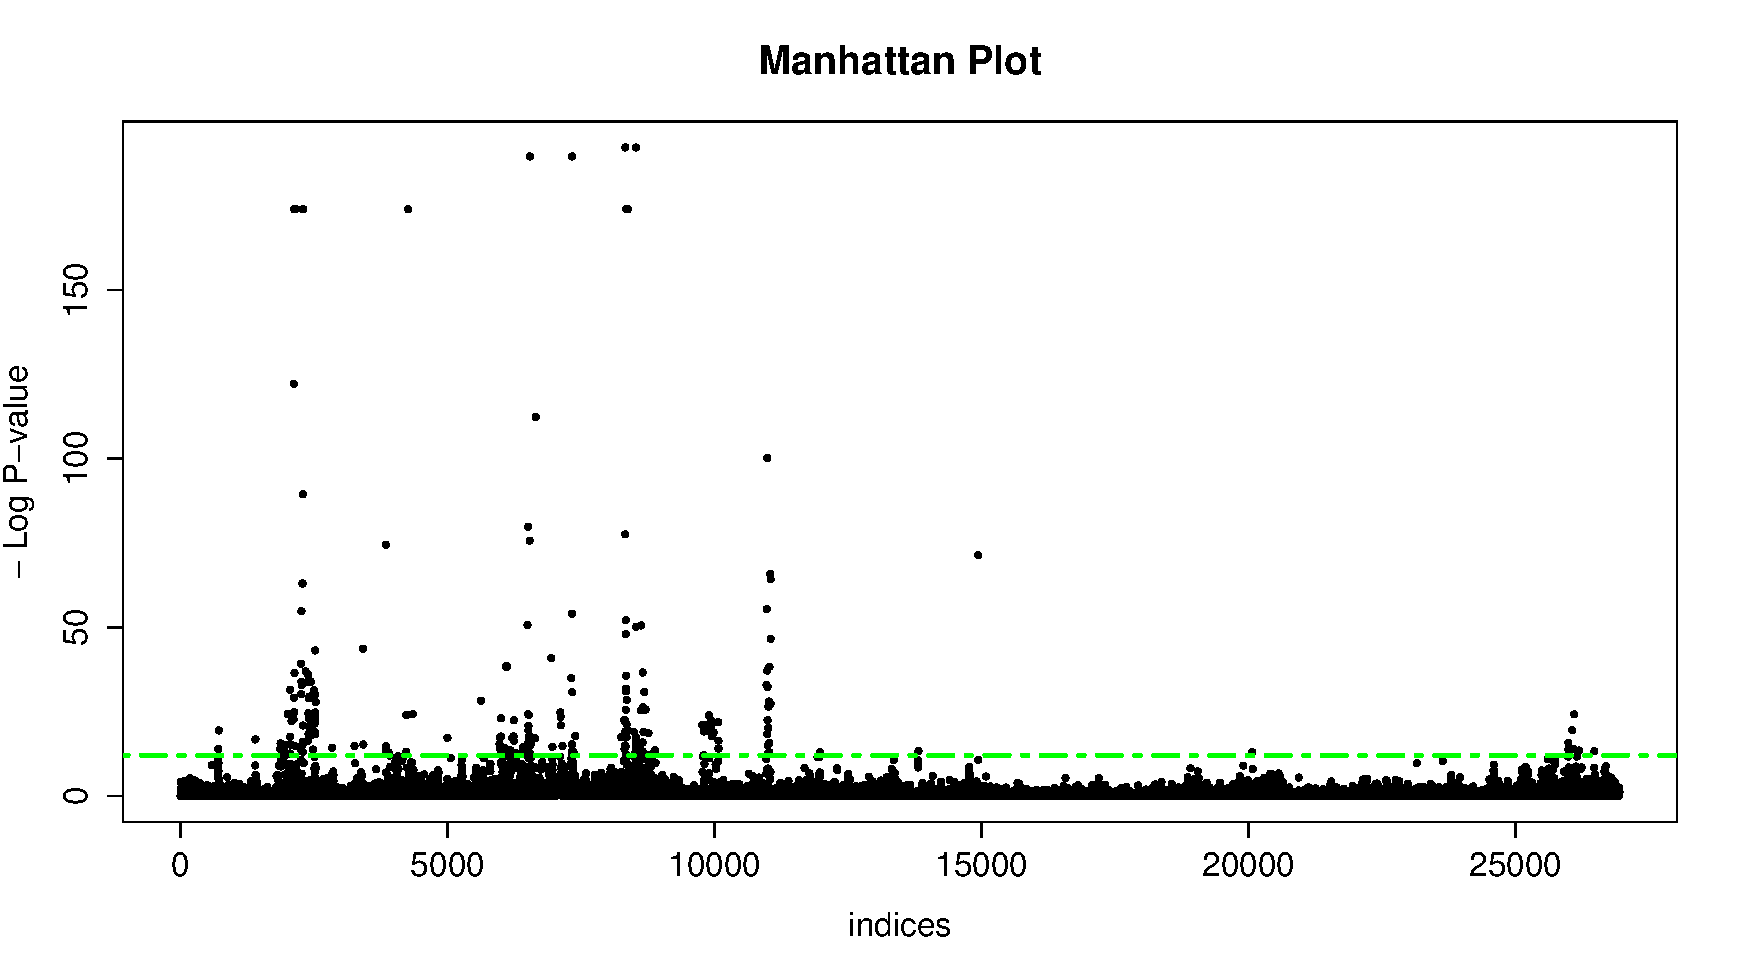
\includegraphics[width=\linewidth]{manhattanPlot.pdf}
\caption{Graph generated with the R script of section~\ref{sec:sel}.}\label{fig:manhattanPlot}
\end{figure} 

\section{Contact}
If you need assistance, do not hesitate to send us an email (kevin.caye@imag.fr or olivier.francois@imag.fr). 

\bibliographystyle{plain}
\bibliography{note}

\end{document}
